%%%%%%%%%%%%%%%%%%%% book.tex %%%%%%%%%%%%%%%%%%%%%%%%%%%%%
%
% sample root file for the chapters of your "monograph"
%
% Use this file as a template for your own input.
%
%%%%%%%%%%%%%%%% Springer-Verlag %%%%%%%%%%%%%%%%%%%%%%%%%%


% RECOMMENDED %%%%%%%%%%%%%%%%%%%%%%%%%%%%%%%%%%%%%%%%%%%%%%%%%%%
\documentclass[pdftex,12pt, oneside]{book}
 
% choose options for [] as required from the list
% in the Reference Guide, Sect. 2.2
%\usepackage[paperwidth=8.5in, paperheight=13in]{geometry} %Folio
\usepackage[paperwidth=8.27in, paperheight=11.69in]{geometry} %A4

\usepackage{makeidx}         % allows index generation
\usepackage{graphicx}        % standard LaTeX graphics tool
                             % when including figure files
\usepackage[bottom]{footmisc}% places footnotes at page bottom
\usepackage[bahasa]{babel}
\usepackage{enumerate}
\usepackage{paralist}
\usepackage{float}
\usepackage{gensymb}  
\usepackage{listings}
\usepackage{color}
\renewcommand{\baselinestretch}{1.5}

\newcommand{\HRule}{\rule{\linewidth}{0.5mm}}

\makeindex             % used for the subject index
                       % please use the style svind.ist with
                       % your makeindex 
                     
\definecolor{codegreen}{rgb}{0,0.6,0}
\definecolor{codegray}{rgb}{0.5,0.5,0.5}
\definecolor{codepurple}{rgb}{0.58,0,0.82}
\definecolor{backcolor}{rgb}{0.95,0.95,0.92}

\lstdefinestyle{mystyle}{
  backgroundcolor=\color{backcolor},
  commentstyle=\color{codegreen},
  keywordstyle=\color{magenta},
  stringstyle=\color{codepurple},
  basicstyle=\footnotesize,
  breakatwhitespace=false,
  breaklines=true,
  captionpos=b,
  keepspaces=true,
  numbers=left,
  numbersep=5pt,
  showspaces=false,
  showstringspaces=false,
  showtabs=false,
  tabsize=2
}

\lstset{style=mystyle}


%%%%%%%%%%%%%%%%%%%%%%%%%%%%%%%%%%%%%%%%%%%%%%%%%%%%%%%%%%%%%%%%%%%%%

\begin{document}
\sloppy


\begin{titlepage}

\begin{center}
{\large DOKUMENTASI RANCANGAN SISTEM BASIS DATA UNTUK SISTEM INFORMASI PEMBAYARAN PAJAK BUMI DAN BANGUNAN PERDESAAN DAN PERKOTAAN DI KABUPATEN BREBES}

\HRule\\[1cm]

PERIODE PENILAIAN TAHUN 2018\\[1cm]


\includegraphics[width=0.5\textwidth]{./resources/logo}\\[1cm]

Oleh :\\
Priyanto Tamami, S.Kom.\\
NIP 19840409 201001 1 025\\


\vfill


Fungsional Pranata Komputer\\
Badan Pengelolaan Pendapatan, Keuangan dan Aset Daerah\\
Pemerintah Daerah Kabupaten Brebes\\
Brebes, 19 Maret 2018
\end{center}

\end{titlepage}

\frontmatter%%%%%%%%%%%%%%%%%%%%%%%%%%%%%%%%%%%%%%%%%%%%%%%%%%%%%%


\begin{center}
{\huge \bfseries Lembar Pengesahan}\\[0.4cm]

\begin{tabular}{l c p{10cm}}
  Nama Kegiatan & : & 	Membuat Petunjuk Operasional Sistem Komputer \\
  Judul & : & PETUNJUK PENGOPERASIAN PROGRAM SISTEM INFORMASI PEMBAYARAN PAJAK BUMI DAN BANGUNAN PERDESAAN DAN PERKOTAAN DI KABUPATEN BREBES \\
\end{tabular}\\[2cm]

\begin{tabular}{c c}
  Disetujui oleh : & Disusun Oleh \\
  Kepala Sub Bidang Keberatan & Pranata Komputer \\
  Pada tanggal 18 April 2018 & Selesai tanggal : 17 April 2018 \\
  & \\
  & \\
  & \\
  M.L. Setiyawan, S.E.Ak & Priyanto Tamami, S.Kom \\
  NIP 19790530 200604 1 006 & NIP 19840409 201001 1 025
\end{tabular}

\end{center}  

\tableofcontents
\listoffigures

\mainmatter%%%%%%%%%%%%%%%%%%%%%%%%%%%%%%%%%%%%%%%%%%%%%%%%%%%%%%%
<<<<<<< HEAD
\chapter{CAKUPAN DAN TUJUAN PROGRAM}

Tujuan dari dibangunnya atau dibentuknya program atau sistem informasi pembayaran pajak bumi dan bangunan sektor perdesaan dan perkotaan ini yaitu untuk menampilkan informasi pencatatan pembayaran yang telah dilakukan oleh wajib pajak, baik yang dilakukan langsung ke Bank sebagai tempat pembayaran, atau ke perangkat Desa/Kelurahan yang nantinya akan disetorkan juga ke Bank sebagai tempat pembayaran.

Dengan kondisi seperti ini, wajib pajak mengetahui bahwa pembayaran yang telah dilakukan sudah diterima oleh rekening Kas Daerah dan tercatat, walaupun pencatatan pembayaran ini memiliki jeda H+1 setelah wajib pajak melakukan pembayaran ke Bank sebagai tempat pembayaran, namun apabila wajib pajak melakukan pembayaran ke petugas pemungut pada tingkat Desa/Kelurahan, maka jeda waktunya akan amat bervariasi bergantung kondisi kapan petugas pemungut tersebut melakukan penyetoran hasil penerimaannya ke Bank sebagai tempat pembayaran.

Dari tujuan tersebut, maka cakupan dari program atau sistem informasi ini sangat sederhana, yaitu menampilkan status pencatatan pembayaran yang telah dicatatkan pada SISMIOP (Sistem Manajemen Informasi Objek Pajak).
\chapter{STRUKTUR DATA / BASIS DATA}

Karena pencatatan pembayaran dari Bank Kas Daerah tercatat pada sistem informasi atau aplikasi SISMIOP (Sistem Manajemen Informasi Objek Pajak), maka struktur basis data yang digunakan pada sistem informasi pembayaran Pajak Bumi dan Bangunan sektor Perdesaan dan Perkotaan menggunakan beberapa tabel pada aplikasi SISMIOP (Sistem Manajemen Informasi Objek Pajak). Tabel-tabel yang digunakan adalah seperti berikut ini :

\section{Tabel SPPT}

Tabel ini selain mencatatkan ketetapan untuk tiap objek pajak pada tiap tahun pajak, tabel ini juga mencatatkan status pembayaran apakah sudah lunas atau belum. Struktur tabelnya adalah seperti pada gambar \ref{fig:struktur-sppt} berikut ini :

\begin{figure}[H]
	\centering
	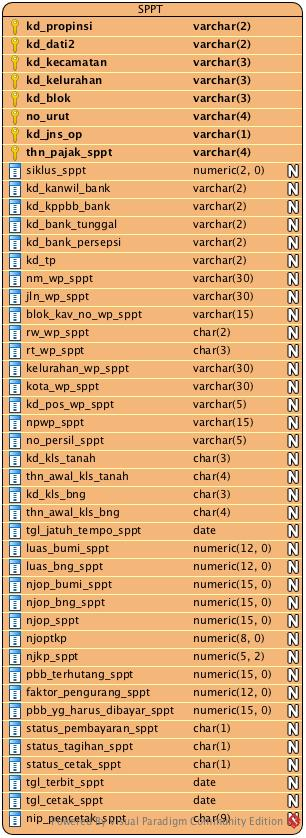
\includegraphics[width=0.5\textwidth]{./resources/struktur-tabel-sppt}
	\caption{Struktur Tabel \texttt{SPPT}}
	\label{fig:struktur-sppt}
\end{figure}

Dari struktur tabel \texttt{SPPT} di atas, beberapa \textit{field} atau kolom yang digunakan pada sistem informasi atau aplikasi ini adalah seperti berikut :

\begin{itemize}
	\item Nomor Objek Pajak, yang terdiri dari \textit{field} atau kolom \texttt{kd\_propinsi}, \texttt{kd\_dati2}, \texttt{kd\_kecamatan}, \texttt{kd\_kelurahan}, \texttt{kd\_blok}, \texttt{no\_urut}, dan \texttt{kd\_jns\_op}.
	\item Tahun pajak pada \textit{field} atau kolom \texttt{thn\_pajak\_sppt}.
	\item Nama wajib pajak pada \textit{field} atau kolom \texttt{nm\_wp\_sppt}
	\item Besarnya pajak terhutang pada \textit{field} atau kolom \texttt{pbb\_yg\_harus\_dibayar\_sppt}
	\item Status pembayaran pada \textit{field} atau kolom \texttt{status\_pembayaran\_sppt}
\end{itemize}

\section{Tabel DAT\_OBJEK\_PAJAK}

Tabel \texttt{DAT\_OBJEK\_PAJAK}, digunakan untuk menampilkan informasi mengenai objek pajak seperti alamat, luas bumi dan bangunan, serta Nilai Jual Objek Bumi dan Bangunan. Struktur tabel dari \texttt{DAT\_OBJEK\_PAJAK} adalah seperti pada gambar \ref{fig:struktur-dat-op} berikut ini :

\begin{figure}[H]
	\centering
	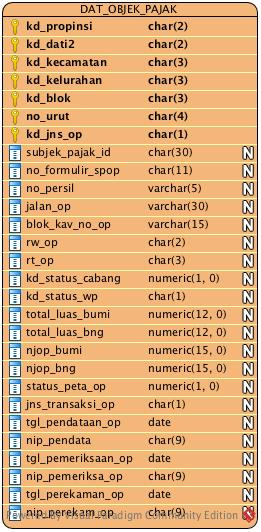
\includegraphics[width=0.5\textwidth]{./resources/struktur-tabel-dat-op}
	\caption{Struktur Tabel \texttt{DAT\_OBJEK\_PAJAK}}
	\label{fig:struktur-dat-op}
\end{figure}

Informasi yang digunakan pada tabel \texttt{DAT\_OBJEK\_PAJAK} ini ada di beberapa \textit{field} atau kolom seperti berikut :

\begin{itemize}
	\item Alamat, akan menggunakan gabungan dari \textit{field} atau kolom \texttt{jalan\_op}, \texttt{blok\_kav\_no\_op}, \texttt{rw\_op}, dan \texttt{rt\_op}.
	\item Luas bumi akan menggunakan \textit{field} atau kolom \texttt{total\_luas\_bumi}.
	\item Luas bangunan akan menggunakan \textit{field} atau kolom \texttt{total\_luas\_bng}.
	\item Nilai Jual Objek Pajak (NJOP) bumi akan menggunakan \textit{field} atau kolom \texttt{njop\_bumi}.
	\item Nilai Jual Objek Pajak (NJOP) bangunan akan menggunakan \textit{field} atau kolom \texttt{njop\_bng}.
\end{itemize}

\section{Tabel DAT\_SUBJEK\_PAJAK}

Tabel \texttt{DAT\_SUBJEK\_PAJAK} ini digunakan untuk menampilkan informasi mengenai subjek pajak seperti nama dan alamatnya. Struktur tabel dari \texttt{DAT\_SUBJEK\_PAJAK} ini adalah seperti pada gambar \ref{fig:struktur-dat-sp} berikut ini :

\begin{figure}[H]
	\centering
	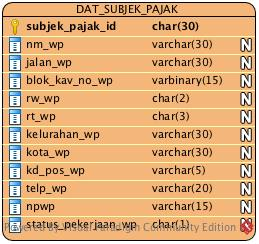
\includegraphics[width=0.5\textwidth]{./resources/struktur-tabel-dat-sp}
	\caption{Struktur Tabel \texttt{DAT\_SUBJEK\_PAJAK}}
	\label{fig:struktur-dat-sp}
\end{figure}

Informasi pada tabel \texttt{DAT\_SUBJEK\_PAJAK} yang digunakan ada pada beberapa \textit{field} atau kolom berikut :

\begin{itemize}
	\item Nama subjek pajak pada \textit{field} atau kolom \texttt{nm\_wp}
	\item Alamat subjek pajak pada \textit{field} atau kolom \texttt{jalan\_wp}, \texttt{blok\_kav\_no\_wp}, \texttt{rw\_wp}, \texttt{rt\_wp}, \texttt{kelurahan\_wp}, dan \texttt{kota\_wp}.
\end{itemize}

\section{Tabel REF\_KECAMATAN}

Untuk tabel \texttt{REF\_KECAMATAN} digunakan hanya untuk menampilkan informasi nama Kecamatan dimana objek berada. Struktur tabel untuk \texttt{REF\_KECAMATAN} ini seperti terlihat pada gambar \ref{fig:struktur-ref-kec} berikut ini :

\begin{figure}[H]
	\centering
	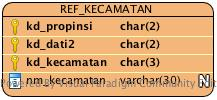
\includegraphics[width=0.5\textwidth]{./resources/struktur-tabel-ref-kec}
	\label{fig:struktur-ref-kec}
	\caption{Struktur Tabel \texttt{REF\_KECAMATAN}}
\end{figure}

Informasi yang digunakan pada tabel \texttt{REF\_KECAMATAN} ini ada pada beberapa \textit{field} atau kolom seperti berikut ini :

\begin{itemize}
	\item Nomor Identifikasi Kecamatan, pada \textit{field} atau kolom \texttt{kd\_propinsi}, \texttt{kd\_dati2}, dan \texttt{kd\_kecamatan}
	\item Nama Kecamatan, pada \textit{field} atau kolom \texttt{nm\_kecamatan}.
\end{itemize}

\section{Tabel REF\_KELURAHAN}

Tabel \texttt{REF\_KELURAHAN} pun digunakan hanya untuk menampilkan nama Kelurahan / Desa dimana objek pajak berada. Struktur tabel \texttt{REF\_KELURAHAN} ini seperti terlihat pada gambar \ref{fig:struktur-ref-kel} berikut ini :

\begin{figure}[H]
	\centering
	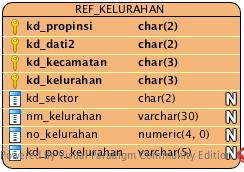
\includegraphics[width=0.5\textwidth]{./resources/struktur-tabel-ref-kel}
	\caption{Struktur Tabel \texttt{REF\_KELURAHAN}}
	\label{fig:struktur-ref-kel}
\end{figure}

Informasi pada tabel \texttt{REF\_KELURAHAN} yang digunakan ada pada beberapa \textit{field} atau kolom berikut ini :

\begin{itemize}
	\item Nomor Identifikasi Kelurahan / Desa pada \textit{field} atau kolom \texttt{kd\_propinsi}, \texttt{kd\_dati2}, \texttt{kd\_kecamatan}, dan \texttt{kd\_kelurahan}.
	\item Nama Desa / Kelurahan pada \textit{field} atau kolom \texttt{nm\_kelurahan}
\end{itemize}
\chapter{FUNGSI-FUNGSI YANG HARUS DILAKUKAN OLEH PROGRAM}

Fungsi yang harus dilakukan oleh program atau sistem informasi yang akan dibangun tentunya harus dapat menampilkan beberapa informasi seperti berikut ini :

\begin{itemize}
	\item Data objek pajak sebagai bahan konfirmasi dan verifikasi bahwa data dengan Nomor Objek Pajak (NOP) yang diinginkan oleh pengguna benar, termasuk di dalamnya adalah Nomor Objek Pajak (NOP), luas bumi dan bangunan, Nilai Jual Objek Pajak Bumi dan Bangunan seperti tertera dalam lembar Surat Pemberitahuan Pajak Terhutang (SPPT), serta lokasi objek pajak berada.
	\item Data subjek pajak, ini pun sebagai bahan konfirmasi dan verifikasi bahwa data subjek pajak yang nantinya ditetapkan sebagai wajib pajak adalah benar seperti tercantum dalam lembar Surat Pemberitahuan Pajak Terhutang (SPPT). Termasuk di dalamnya adalah data-data seperti nomor identitas subjek pajak, nama subjek pajak, serta alamat tempat tinggal subjek pajak.
	\item Data tagihan dari Surat Pemberitahuan Pajak Terhutang (SPPT) yang ditampilkan secara rinci untuk tiap tahun pajak. Termasuk di dalamnya adalah informasi mengenai tahun pajak, besarnya tagihan terhutang, dan status pembayaran yang tercatat.
\end{itemize}
\chapter{BATASAN DAN KARAKTERISTIK KINERJA PROGRAM}

\section{Batasan Program}

Batasan dari program atau sistem informasi yang dibangun ini adalah bahwa aplikasi atau program atau sistem informasi ini, sesuai dengan tujuannya, yaitu menampilkan informasi status pencatatan pembayaran dari Sistem Manajemen Informasi Objek Pajak (SISMIOP) adalah sebatas memberikan informasi status pencatatan pembayaran yang telah terjadi berdasarkan Nomor Objek Pajak (NOP) yang tertera pada lembar Surat Pemberitahuan Pajak Terhutang (SPPT) yang diberikan tiap tahunnya.

Aplikasi atau program atau sistem informasi yang dibangun tidak mampu untuk melakukan perubahan pencatatan pembayaran, atau perubahan-perubahan terhadap data yang ditayangkan, untuk perubahan-perubahan atau manipulasi data terhadap data yang tampil dilakukan dengan aplikasi lain, yaitu Sistem Manajemen Informasi Objek Pajak (SISMIOP) yang digunakan untuk melakukan pengelolaan data-data objek pajak bumi dan bangunan sektor perdesaan dan perkotaan.

\section{Karakteristik Kinerja Program}

Karakteristik kinerja dari program atau aplikasi atau sistem informasi yang dibangun, karena menggunakan skema aplikasi dengan 2 (dua) lapis, yaitu bagian ujung-belakang (\textit{backend}) dan bagian ujung-depan (\textit{frontend}), sehingga program atau aplikasi ini dapat lebih mudah untuk dikembangkan ke aplikasi model lain seperti aplikasi \textit{mobile} dengan basis Android atau iOS, atau bahkan dikembangkan menjadi aplikasi berbasis \textit{desktop}.

Komunikasi yang terjadi antara 2 (dua) bagian ini adalah melalui arsitektur REST (\textit{Representational State Transfer}), dimana peladen akan menyediakan \textit{resources} (sumber daya / data) dan klien akan melakukan akses dan menampilkan \textit{resource} tersebut. \textit{Resource} atau sumber daya ini akan dikirimkan oleh peladen dalam format JSON untuk mempermudah melakukan penguraian datanya.
\chapter{KRITERIA PENGUJIAN PROGRAM}

Kriteria yang diperlukan untuk melakukan pengujian kesesuaian program terhadap spesifikasi, karena akan menggunakan \textit{unit test} dan \textit{integration test}, maka beberapa poin kriterianya adalah seperti berikut ini :

\begin{itemize}
	\item Pengujian terhadap data objek pajak :
	
	\begin{itemize}
		\item Nomor objek pajak yang dikembalikan dari sistem basis data harus sesuai seperti data yang dikirimkan saat klien melakukan \textit{request}.
		\item Luas bumi yang dihasilkan berdasarkan Nomor Objek Pajak tertentu harus sama besarnya seperti yang tertera dalam sistem basis data.
		\item Luas bangunan yang dihasilkan berdasarkan Nomor Objek Pajak tertentu harus sama besarnya seperti yang tertera dalam sistem basis data.
		\item Nilai jual objek pajak bumi yang dihasilkan berdasarkan Nomor Objek Pajak tertentu harus sama besarnya seperti yang tertera dalam sistem basis data.
		\item Nilai jual objek pajak bangunan yang dihasilkan berdasarkan Nomor Objek Pajak tertentu harus sama besarnya seperti yang tertera dalam sistem basis data.
		\item Nama jalan yang dihasilkan berdasarkan Nomor Objek Pajak tertentu harus sama nilainya seperti yang tertera dalam sistem basis data.
		\item Nomor blok, atau nomor rumah yang dihasilkan berdasarkan Nomor Objek Pajak harus sama nilainya seperti yang tertera dalam sistem basis data.
		\item Nomor RT yang dihasilkan berdasarkan Nomor Objek Pajak tertentu harus sama nilainya seperti yang tertera dalam sistem basis data.
		\item Nomor RW yang dihasilkan berdasarkan Nomor Objek Pajak tertentu harus sama nilainya seperti yang tertera dalam sistem basis data.
		\item Nama Kecamatan yang dihasilkan berdasarkan Nomor Objek Pajak tertentu harus sama seperti yang tertera dalam sistem basis data.
		\item Nama Kelurahan / Desa yang dihasilkan berdasarkan Nomor Objek Pajak tertentu harus sama seperti yang tertera dalam sistem basis data.
	\end{itemize}
	
	\item Pengujian terhadap data subjek pajak :
	
	\begin{itemize}
		\item Nama subjek pajak yang dihasilkan berdasarkan Nomor Objek Pajak tertentu, hasilnya harus sama seperti yang tertera dalam sistem basis data.
		\item Nama jalan tempat subjek pajak tinggal yang dihasilkan berdasarkan Nomor Objek Pajak tertentu, hasilnya harus sama seperti yang tertera dalam sistem basis data.
		\item Nomor blok atau nomor rumah tempat subjek pajak tinggal yang dihasilkan berdasarkan Nomor Objek Pajak tertentu, hasilnya harus sama seperti yang tertera dalam sistem basis data.
		\item Nomor RT tempat subjek pajak tinggal yang dihasilkan berdasarkan Nomor Objek Pajak tertentu, hasilnya harus sama seperti yang tertera dalam sistem basis data.
		\item Nomor RW tempat subjek pajak tinggal yang dihasilkan berdasarkan Nomor Objek Pajak tertentu, harus sama seperti yang tertera dalam sistem basis data.
		\item Nama Kelurahan / Desa tempat subjek pajak tinggal berdasarkan Nomor objek Pajak tertentu, isinya harus sama seperti yang tertera dalam sistem basis data.
		\item Nama Kota tempat subjek pajak tinggal berdasarkan Nomor Objek Pajak tertentu, isinya harus sama seperti yang tertera dalam sistem basis data.
	\end{itemize}
	
	\item Pengujian terhadap data tagihan dari Surat Pemberitahuan Pajak Terhutang (SPPT) untuk tiap tahun pajak : 
	
	\begin{itemize}
		\item Besarnya pajak terhutang untuk setiap tahun pajak berdasarkan Nomor objek Pajak tertentu, harus sama nilanya seperti kondisi pada sistem basis data.
		\item Kondisi status pembayaran untuk setiap tahun pajak berdasarkan Nomor Objek Pajak tertentu, harus sama nilanya seperti kondisi pada sistem basis data.
	\end{itemize}
\end{itemize}
=======
\chapter{PROSEDUR VERIFIKASI / VALIDASI SPESIFIKASI PROGRAM}

Prosedur verifikasi atas spesifikasi program akan dilakukan saat pengembangan aplikasi / program dengan \textit{unit testing} dan \textit{integration testing}.

Data yang digunakan untuk pengembangan dan pengujian dilakukan dengan data \textit{dummy} menggunakan struktur data asli seperti pada spesifikasi sistem basis data.

\textit{Unit testing} dan \textit{integration testing} yang dilakukan akan terbagi menjadi beberapa kelompok seperti spesifikasi berikut :

\section{Pengujian Permintaan Terhadap Objek Pajak}

\subsection{Nomor Objek Pajak}

Pada saat klien melakukan permintaan data ke peladen, hal pertama yang dilakukan adalah memeriksa kebenaran Nomor Objek Pajak (NOP) yang sampai ke peladen, apakah Nomor Objek Pajak yang dikirimkan oleh klien, telah diterima benar susunannya pada peladen.

Pemeriksaan ini dilakukan pada objek \texttt{JsonObject}. Apabila \textit{method} \texttt{setNop()} berisi parameter berupa Nomor Objek Pajak (NOP) \texttt{332901000100500390}, maka \textit{method} \texttt{getNop()} harus memberikan hasil yang sama.

\subsection{Luas Bumi Objek Pajak}

Pada bagian ini, klien akan melakukan \textit{request} atau permintaan data ke peladen dengan membawa parameter \texttt{keyword} berisi \texttt{op}, dan \texttt{nop} berisi \texttt{332901000100500390}.	

Hasil dari \textit{request} atau permintaan terhadap API (\textit{application programmable interface}) ini berupa data bertipe \texttt{BigDecimal} dengan nilai \texttt{80} untuk luas bumi objek pajaknya.

\subsection{Luas Bangunan Objek Pajak}

Pada bagian ini, klien masih melakukan \textit{request} atau permintaan data ke peladen dengan membawa parameter \texttt{keyword} berisi \texttt{op}, dan \texttt{nop} berisi \texttt{332901000100500390}.

Hasil dari \textit{request} atau permintaan terhadap API (\textit{Application Programmable Interface}) ini berupa data bertipe \texttt{BigDecimal} dengan nilai \texttt{40} untuk luas bangunan objek pajaknya.

\subsection{NJOP Bumi Objek Pajak}

Pada bagian ini, klien masih melakukan \textit{request} atau permintaan data ke peladen dengan parameter yang sama, yaitu \texttt{keyword} yang berisi \texttt{op}, dan \texttt{nop} yang berisi \texttt{332901000100500390}.

Hasil keluaran untuk Nilai Jual Objek Pajak (NJOP) Bumi dari \textit{request} atau permintaan data tersebut akan bertipe \texttt{BigDecimal} dengan nilai \texttt{1600000} (Satu juta enam ratus) rupiah per meter persegi.

\subsection{NJOP Bangunan Objek Pajak}

\textit{Request} untuk bagian ini masih dengan parameter yang sama, yaitu parameter \texttt{keyword} yang berisi \texttt{op}, dan \texttt{nop} yang berisi \texttt{332901000100500390}.

Hasil Nilai Jual Objek Pajak (NJOP) Bangunan yang didapat dari \textit{request} atau permintaan data tersebut bertipe \texttt{BigDecimal} dengan nilai \texttt{9000000} (Sembilan juta) rupiah per meter persegi.

\subsection{Nama Jalan Objek Pajak}

Untuk pengambilan nama jalan dari objek pajak, masih menggunakan parameter yang sama untuk \textit{request} atau permintaan data ke peladen, yaitu dengan parameter \texttt{keyword} yang berisi \texttt{op}, dan \texttt{nop} yang berisi \texttt{332901000100500390}.

Hasil yang seharusnya didapat dari \textit{request} atau permintaan data di atas akan memiliki tipe data \texttt{String} dengan nilai \texttt{KP RW 01}.

\subsection{RT dan RW Objek Pajak}

Untuk pengambilan data RT dan RW objek pajak, masih menggunakan parameter yang sama untuk \textit{request} atau permintaan data ke peladen, yaitu dengan parameter \texttt{keyword} yang berisi \texttt{op}, dan \texttt{nop} yang berisi \texttt{332901000100500390}.

Hasil yang seharusnya didapat dari \textit{request} atau permintaan data tersebut akan memiliki tipe data \texttt{string} dengan nilai \texttt{RT. 002 RW. 01}.

\subsection{Nama Kelurahan Objek Pajak}

Pengambilan data nama Kelurahan atau nama Desa untuk objek pajak masih menggunakan parameter yang sama untuk \textit{request} atau permintaan data ke peladen, yaitu dengan parameter \texttt{keyword} yang berisi \texttt{op}, dan \texttt{nop} yang berisi \texttt{332901000100500390}.

Hasil yang seharusnya didapatkan dari \textit{request} atau permintaan data tersebut akan memiliki tipe data \texttt{string} dengan nilai \texttt{GUNUNGJAYA}.

\subsection{Nama Kecamatan Objek Pajak}

Tidak berbeda dengan pengujian sebelumnya, untuk pengambilan data nama Kecamatan sebuah objek pajak masih menggunakan parameter yang sama untuk \textit{request} atau permintaan data ke peladen, yaitu dengan parameter \texttt{keyword} yang berisi \texttt{op}, dan \texttt{nop} yang berisi \texttt{332901000100500390}.

Hasil yang seharusnya didapatkan dari \textit{request} atau permintaan data tersebut akan memiliki tipe data \texttt{string} dengan nilai \texttt{SALEM}.

\subsection{Nomor Identitas Subjek Pajak}

Untuk pengambilan data nomor identitas subjek pajak pun masih menggunakan parameter \textit{request} atau permintaan data ke peladen berupa parameter \textit{keyword} yang berisi \texttt{op} dan parameter \texttt{nop} yang berisi \texttt{332901000100500390}.

Hasil yang seharusnya didapatkan dari \textit{request} atau permintaan data tersebut akan memiliki tipe data \texttt{string} dengan nilai \texttt{332901000100500390}

\section{Pengujian Permintaan Terhadap Data Subjek Pajak}

Untuk pengujian permintaan terhadap data subjek pajak akan terdiri dari beberapa bagian berikut :

\subsection{Nama Subjek Pajak}

Permintaan data nama subjek pajak dilakukan oleh klien ke peladen API (\textit{Application Programmable Interface}) dengan parameter \texttt{keyword} yang isinya \texttt{wp} dan parameter \texttt{subjek\_pajak\_id} yang berisi nomor identitas dari subjek pajak tersebut, yang diambil sebagai contoh pengujian adalah \texttt{332901000100500390}.

Hasil yang seharusnya didapatkan dari \textit{request} atau permintaan data tersebut berupa nama \texttt{KARSO} dengan tipe data \texttt{string}.

\subsection{Nama Jalan Alamat Subjek Pajak}

Untuk pengujian nama jalan dari alamat subjek pajak, akan dilakukan oleh klien ke peladen dengan \textit{request} parameter berupa \texttt{keyword} dengan nilai \texttt{wp} dan parameter \texttt{subjek\_pajak\_id} dengan nilai \texttt{332901000100500390}.

Hasil yang seharusnya didapatkan dari \textit{request} atau permintaan data tersebut adalah nilai \texttt{KP RW 01} dengan tipe data \texttt{string}.

\subsection{RT dan RW dari Alamat Subjek Pajak}

Untuk pengujian permintaan data RT dan RW dari alamat subjek pajak yang akan dilakukan klien ke peladen adalah menggunakan parameter \texttt{keyword} yang berisi \texttt{wp} dan parameter \texttt{subjek\_pajak\_id} dengan isi \texttt{332901000100500390}.

Hasil yang didapat untuk \textit{request} atau permintaan tersebut seharusnya adalah berupa data \texttt{RT. 002 RW. 01} dengan tipe data \texttt{string}

\subsection{Nama Kelurahan dari Alamat Subjek Pajak}

Untuk pengujian permintaan data nama Kelurahan / Desadari alamat subjek pajak yang akan dilakukan klien ke peladen adalah menggunakan parameter \texttt{keyword} yang berisi \texttt{wp}, dan parameter \texttt{subjek\_pajak\_id} yang berisi \texttt{332901000100500390}.

Hasil yang seharusnya didapat untuk parameter tersebut adalah data \texttt{GUNUNGJAYA} dengan tipe data \texttt{string}.

\subsection{Nama Kota atau Kabupaten dari Alamat Subjek Pajak}

Untuk pengujian permintaan data nama Kota atau Kabupaten dari alamat subjek pajak yang dilakukan klien ke peladen adalah menggunakan parameter \texttt{keyword} yang berisi \texttt{wp}, dan parameter \texttt{subjek\_pajak\_id} yang berisi \texttt{332901000100500390}.

Hasil yang seharusnya didapat untuk parameter tersebut adalah data \texttt{KAB BREBES} dengan tipe data \texttt{string}.

\section{Pengujian Permintaan Data Ketetapan}

Untuk pengujian permintaan data ketetapan tiap tahun pajak, hal yang perlu dilakukan pengujian adalah seperti berikut ini :

\subsection{Pengujian Atas Daftar Ketetapan}

Pengujian atas daftar ketetapan dilakukan klien dengan cara melakukan \textit{request} atau permintaan data ke peladen dengan parameter \texttt{keyword} yang berisi \texttt{sppt}, dan parameter \texttt{nop} yang berisi \texttt{332901000100500390}.

Hasil yang seharusnya dikembalikan oleh peladen adalah berupa daftar tahun pajak dimana Nomor Objek Pajak tersebut telah terbit sebagai Surat Pemberitahuan Pajak Terhutang (SPPT) untuk tiap tahun pajak, adapun banyaknya data yang seharusnya ditampilkan untuk Nomor Objek Pajak (NOP) tersebut adalah 8 (delapan data).

\subsection{Pengujian Besarnya NIlai Pajak Terhutang Tiap Tahun Pajak}

Untuk pengujian besarnya nilai pajak, akan menggunakan 3 (tiga) contoh data seperti berikut :

\begin{itemize}
	\item \textit{Request} pertama menggunakan parameter \texttt{keyword} yang berisi \texttt{bayar}, parameter \texttt{nop} yang berisi \texttt{332911090400000967}, dan parameter \texttt{tahun} yang berisi \texttt{1994}. Hasil yang diharapkan dari \textit{request} ini adalah data \texttt{2088} dengan tipe data \texttt{BigDecimal}.
	\item \textit{Request} yang kedua menggunakan parameter \texttt{keyword} yang berisi \texttt{bayar}, parameter \texttt{nop} yang berisi \texttt{332912090500003797}, dan parameter \texttt{tahun} yang berisi \texttt{1994}. Hasil yang diharapkan dari \textit{request} ini adalah data \texttt{2720} yang bertipe \texttt{BigDecimal}.
	\item \textit{Request} yang ketiga menggunakan parameter \texttt{keyword} yang berisi \texttt{bayar}, parameter \texttt{nop} yang berisi \texttt{332912090500003657}. Hasil yang diharapkan dari \textit{request} ini adalah data \texttt{3920} dengan tipe data \texttt{BigDecimal}.
\end{itemize}

\subsection{Pengujian Status Pembayaran Untuk Tiap Tahun Pajak}

Untuk pengujian status pembayaran untuk tiap tahun pajak akan menggunakan 1 (satu) contoh data dalam 1 (satu) kali \textit{request}, dan akan dicocokan datanya dengan 3 (tiga) tahun pertama terbit, apakah statusnya sudah \texttt{LUNAS} atau \texttt{BELUM LUNAS}.

\textit{Request} yang dilakukan klien ke peladen menggunakan parameter \texttt{keyword} yang berisi \texttt{sppt} dan parameter \texttt{nop} dengan isi \texttt{332901000100500390}. Hasil yang diharapkan untuk data pertama, data kedua, dan data ketiga dari daftar yang diberikan oleh peladen harus bernilai \texttt{LUNAS}.

\section{Pengujian Modul \textit{Service}}

Pengujian atas \textit{service} yang terbentuk akan terbagi menjadi 3 (tiga) bagian seperti jumlah kelas yang terdapat pada paket \texttt{service} seperti berikut :

\subsection{Pengujian Terhadap Kelas \texttt{DatObjekPajakService}}

Pada pengujian kali ini, yang digunakan adalah 1 (satu) buah contoh data berdasarkan Nomor Objek Pajak (NOP), nantinya data yang dikembalikan dari sistem basis data harus memenuhi nilai yang ditentukan. \textit{Request} yang dilakukan adalah terhadap Nomor Objek Pajak (NOP) \texttt{332901000100500390}, hasil yang diharapkan adalah sebuah objek \texttt{DatObjekPajakModif} dengan nilai berikut :

\begin{itemize}
	\item Atribut \texttt{op\_kec} seharusnya bernilai \texttt{SALEM} dengan tipe data \texttt{string}
	\item Atribut \texttt{op\_kel} seharusnya bernilai \texttt{GUNUNGJAYA} dengan tipe data \texttt{string}
	\item Atribut \texttt{op\_jalan} seharusnya bernilai \texttt{KP RW 01} dengan tipe data \texttt{string}
	\item Atribut \texttt{op\_rtrw} seharusnya bernilai \texttt{RT. 002 RW. 01} dengan tipe data \texttt{string}
	\item Atribut \texttt{op\_luas\_bumi} seharusnya bernilai \texttt{80} dengan tipe data \texttt{BigDecimal}
	\item Atribut \texttt{op\_luas\_bng} seharusnya bernilai \texttt{40} dengan tipe data \texttt{BigDecimal}
	\item Atribut \texttt{op\_njop\_bumi} seharusnya bernilai \texttt{1600000} dengan tipe data \texttt{BigDecimal}
	\item Atribut \texttt{op\_njop\_bng} seharusnya bernilai \texttt{9000000} dengan tipe data \texttt{BigDecimal}
	\item Atribut \texttt{op\_wp\_id} seharusnya bernilai \texttt{332901000100500390} dengan tipe data \texttt{string}
\end{itemize}

\subsection{Pengujian Terhadap Kelas \texttt{DatSubjekPajakService}}

Pengujian terhadap kelas \texttt{DatSubjekPajak} pun akan dilakukan dengan sebuah parameter berupa nomor identitas subjek pajak dengan nilai \texttt{332901000100500390}. Hasil yang seharusnya didapatkan adalah objek dari kelas \texttt{DatSubjekPajakModif} dengan rincian nilai atas atribut seperti berikut ini :

\begin{itemize}
	\item Atribut \texttt{wp\_nama} dengan isi \texttt{KARSO} dengan tipe data \texttt{string}
	\item Atribut \texttt{wp\_jalan} dengan isi \texttt{KP RW 01} dengan tipe data \texttt{string}
	\item Atribut \texttt{wp\_rtrw} dengan isi \texttt{RT. 002 RW. 01} dengan tipe data \texttt{string}
	\item Atribut \texttt{wp\_kel} dengan isi \texttt{GUNUNGJAYA} dengan tipe data \texttt{string}
	\item Atribut \texttt{wp\_kota} dengan isi \texttt{KAB BREBES} dengan tipe data \texttt{string}
\end{itemize}

\subsection{Pengujian Terhadap Kelas \texttt{SpptService}}

Untuk pengujian kelas \texttt{SpptService}, yang akan diuji adalah hasil dari \textit{method} \texttt{getSppt()} dan \texttt{getPiutang()}

Pada saat pemanggilan \textit{method} \texttt{getSppt()} dengan menggunakan parameter Nomor Objek Pajak (NOP) \texttt{332901000100500390}, maka \textit{method} tersebut akan mengembalikan nilai berupa daftar dengan tipe data \texttt{List}, jumlah data yang terdapat pada \texttt{List} ini seharusnya ada 8 (delapan) buah data.

Kemudian pada saat pemanggilan \textit{method} \texttt{getPiutang()} untuk dilakukan uji coba, parameter yang dilewatkan adalah berupa Nomor Objek Pajak (NOP) dengan isi \texttt{332911090400000967}, kemudian parameter kedua diisi dengan tahun pajak, yaitu \texttt{1994}.

Diharapkan hasil dari operasi di atas adalah data \texttt{2088} dengan tipe data berupa \texttt{BigDecimal}.
\chapter{PETUGAS VERIFIKASI ATAU VALIDASI PROGRAM}

Karena pengujian dilakukan secara paralel pada saat pengembangan aplikasi atau program, dan dilakukan secara otomatis dengan kode program, maka kebutuhan untuk petugas verifikasi atau validasi program tidak diperlukan lagi untuk pengembangan sistem informasi atau aplikasi ini.
\chapter{JADWAL PELAKSANAAN}

Jadwal pelaksanaan pengujian akan dilakukan bersamaan pada saat melakukan \textit{coding} program, sehingga dalam siklusnya, saat selesai mengerjakan sebuah fitur dalam program, kode otomasi untuk pengujian akan dibuatkan juga untuk memastikan bahwa program atau aplikasi yang akan di kompilasi telah lulus dari pengujian.
>>>>>>> f6adbf289a5d25679d8a151dafd7a62049e5a3fe

\backmatter%%%%%%%%%%%%%%%%%%%%%%%%%%%%%%%%%%%%%%%%%%%%%%%%%%%%%%%
\printindex

%%%%%%%%%%%%%%%%%%%%%%%%%%%%%%%%%%%%%%%%%%%%%%%%%%%%%%%%%%%%%%%%%%%%%%

\end{document}





